\scanpage{23}
\mspage{22}
\mspage{IV-951}

et il est clair par (18.\unsure{6}.6,(v)) que si $A$ est noethérien \deleted{\unsure{,}}, il en est de même de ${}^h A$.

\deleted{Enfin, ${}^h A$ possède aussi la propriété universelle (18.6.6,(ii)) en convenant d'appeler ``homomorphisme \inserted{semi-}local'' de $A$ dans un anneau \inserted{semi-}local $B$ tout homomorphisme $\varphi$ tel que $\varphi(\underline r)$ soit contenu dans l'idéal maximal \inserted{$\underline n$} de $B$. En effet, il est clair que pour un tel homomorphisme, $\varphi^{-1}(\underline n)$ doit contenir l'un des $\underline m_{\unsure{1|i}}$ puisqu'il contient leur intersection, donc $\varphi^{-1}(\underline n)$ est égal à l'un des $\underline m_{\unsure{1|i}}$, et $\varphi$ se factorise \deleted{\unsure{donc}} en $A\to A_{\underline m_{\unsure{1|i}}}\to B$; d'où l'on conclut \deleted{\illegible{1}} que $\operatorname{Hom.loc}(A,B)\unsure{-|=}\prod_i\operatorname{Hom.loc}(A_{\underline m_{\unsure{1|i}}},B)$, et le fait que (18.6.6,(ii)) est encore valable lorsque $A$ est semi-local en découle aussitôt.}

\margin{\unsure{vider|virer}, (la forme hybride ici ne mérite pas le nom de ``\unsure{prop.} universelle'') ou bien \unsure{arranger} avec des ``hom $\frac12$ locaux'' dans des \unsure{anneaux semi-locaux}}

\uline{Proposition} (18.6.8). -- \uline{Soient $A$ un anneau semi-local, $B$ une $A$-algèbre semi-locale et entière sur $A$. Alors $B\otimes_A({}^h A)$ est une $B$-algèbre semi-locale isomorphe à ${}^h B$.}

\deleted{\illegible{13}} Comme $B\otimes_A({}^h A)$ est entier au-dessus de ${}^h A$, chacun de ses idéaux maximaux est au-dessus d'un des idéaux maximaux de ${}^h A$, donc au-dessus d'un idéal maximal de $A$, et comme $B$ est entière sur $A$, les idéaux premiers de $B$ au-dessus d'un idéal maximal de $A$ sont des idéaux maximaux de $B$, si bien que finalement un idéal maximal de $B\otimes_A({}^h A)$ a pour projections dans $\operatorname{Spec}({}^h A)$ et $\operatorname{Spec}(B)$ des idéaux maximaux; compte tenu de (18.6.6,(iii)) et de (\uline{I},3.4.9), on conclut que l'anneau $B\otimes_A({}^h A)$ est semi-local. En outre, pour tout anneau local hensélien \inserted{$C$}, $\operatorname{Hom.loc}(B\otimes_A({}^h A),C)$ est en correspondance biunivoque avec l'ensemble des couples $(\varphi,\psi)$ d'homomorphismes locaux $\varphi:B\to C$, $\psi:{}^h A\to C$ tels que les composés $A\to B\xrightarrow{\varphi}C$, $A\to{}^h A\xrightarrow{\psi}C$ soient égaux. Mais \deleted{\illegible{4}} en vertu de la correspondance biunivoque entre $\operatorname{Hom.loc}(A,C)$ et $\operatorname{Hom.loc}({}^h A,C)$, on voit que pour tout $\varphi\in\operatorname{Hom.loc}(B,C)$ il existe un $\psi$ et un seul ayant \deleted{les}\inserted{la} propriété\deleted{s} précédente\deleted{s}, donc l'application $\operatorname{Hom}(B\otimes_A({}^h A),C)\to\operatorname{Hom}(B,C)$ est bijective, ce qui prouve la proposition en vertu de l'unicité de la solution
\figure{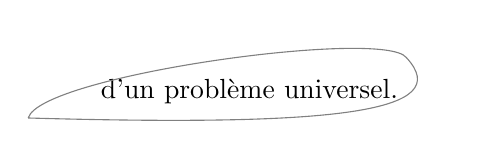
\begin{tikzpicture}[x=1cm,y=1cm]\node[anchor=west] at (0,0) {d'un problème universel.};\draw[gray] (-.8,-.34) .. controls (-.65,.2) and (3.7,.8) .. (4.0,.43) .. controls (4.65,-.27) and (3.1,-.45) .. (-.8,-.34);\end{tikzpicture}}

\margin{\uline{\unsure{Coroll.|cercle}}}

\uline{Théorème} (18.6.9). -- \uline{Soit $A$ un anneau semi-local.}

(i) \uline{Pour que ${}^h A$ soit réduit (resp. normal), il faut et il suffit que $A$ le soit.}

(ii) \uline{Supposons $A$ noethérien. Alors, pour tout idéal premier $\underline p$ de $A$, l'an-}
